\documentclass[../thesis/thesis.tex]{subfiles}
\begin{document}
 \chapter{Evaluation}
 \label{chap:evaluation}

 With a sensing system design determined and constructed, we are now able to perform experiments involving the system. In this chapter we create a set of experiments to test the sensor system's properties and come to conclusions as to their effect on our ability to detect occupants. We then outline a process for taking raw sensor data and performing occupancy predictions with it. Using that process, we then devise a set of occupancy scenarios, and experiment with different machine learning algorithms abilities to determining occupancy from that data.

\section{Sensor Properties}

In order to best utilize the \mlx, we must first understand the properties it exhibits, and their potential effects on our ability to perform occupancy measurements. These properties can be broadly separated into three different categories; bias, noise and sensitivity.

\subsection{Bias}
When detecting no infrared radiation (IR), the sensor should indicate a near-zero temperature, as the sensor's method of determining temperature involves measuring IR. If in such conditions the temperatures indicated are non-uniform, that suggests that the sensor has some level of bias in its measurements. We attempted to investigate the possibility of such bias by performing thermal captures of the night sky. While this does not completely eliminate the IR, it does remove a significant proportion of it.

To test this, the thermal sensor was exposed to the night sky at a capture rate of 1Hz for 4 minutes, with the sensing results combined to create a set of means and standard deviations for the pixels at ``rest''. The average temperature detected was $11.78\dc$, with the standard deviation remaining less than $0.51\dc$ over the entire exposure period. The resultant mean thermal map (\Fref{fig:meanplot}) shows that the four center pixels maintain a similar temperature around $9\dc$, with temperatures beginning to deviate as they became further from that point.

The most likely cause of this bias is related to the physical structure of the sensor. The \mlx is a rectangular sensor which has been placed inside a circular tube. Due to this physical arrangement, the sides of this rectangular sensor will be significantly closer to these edges than the center. If the sensor's casing is at an ambient temperature higher than the measurement data (as they likely were in this case) thermal radiation from the sensor package itself could provide significant enough to cause the edges to appear warmer than the observed area of the sky. This effect could be controlled for by cooling the sensor package to below that of the ambient temperature being measured, however, this is not a concern in this project, as the method of calculating a thermal background will compensate for any such bias provided it remains relatively constant, which if our hypothesis is correct, it should.

\begin{figure}
\centering
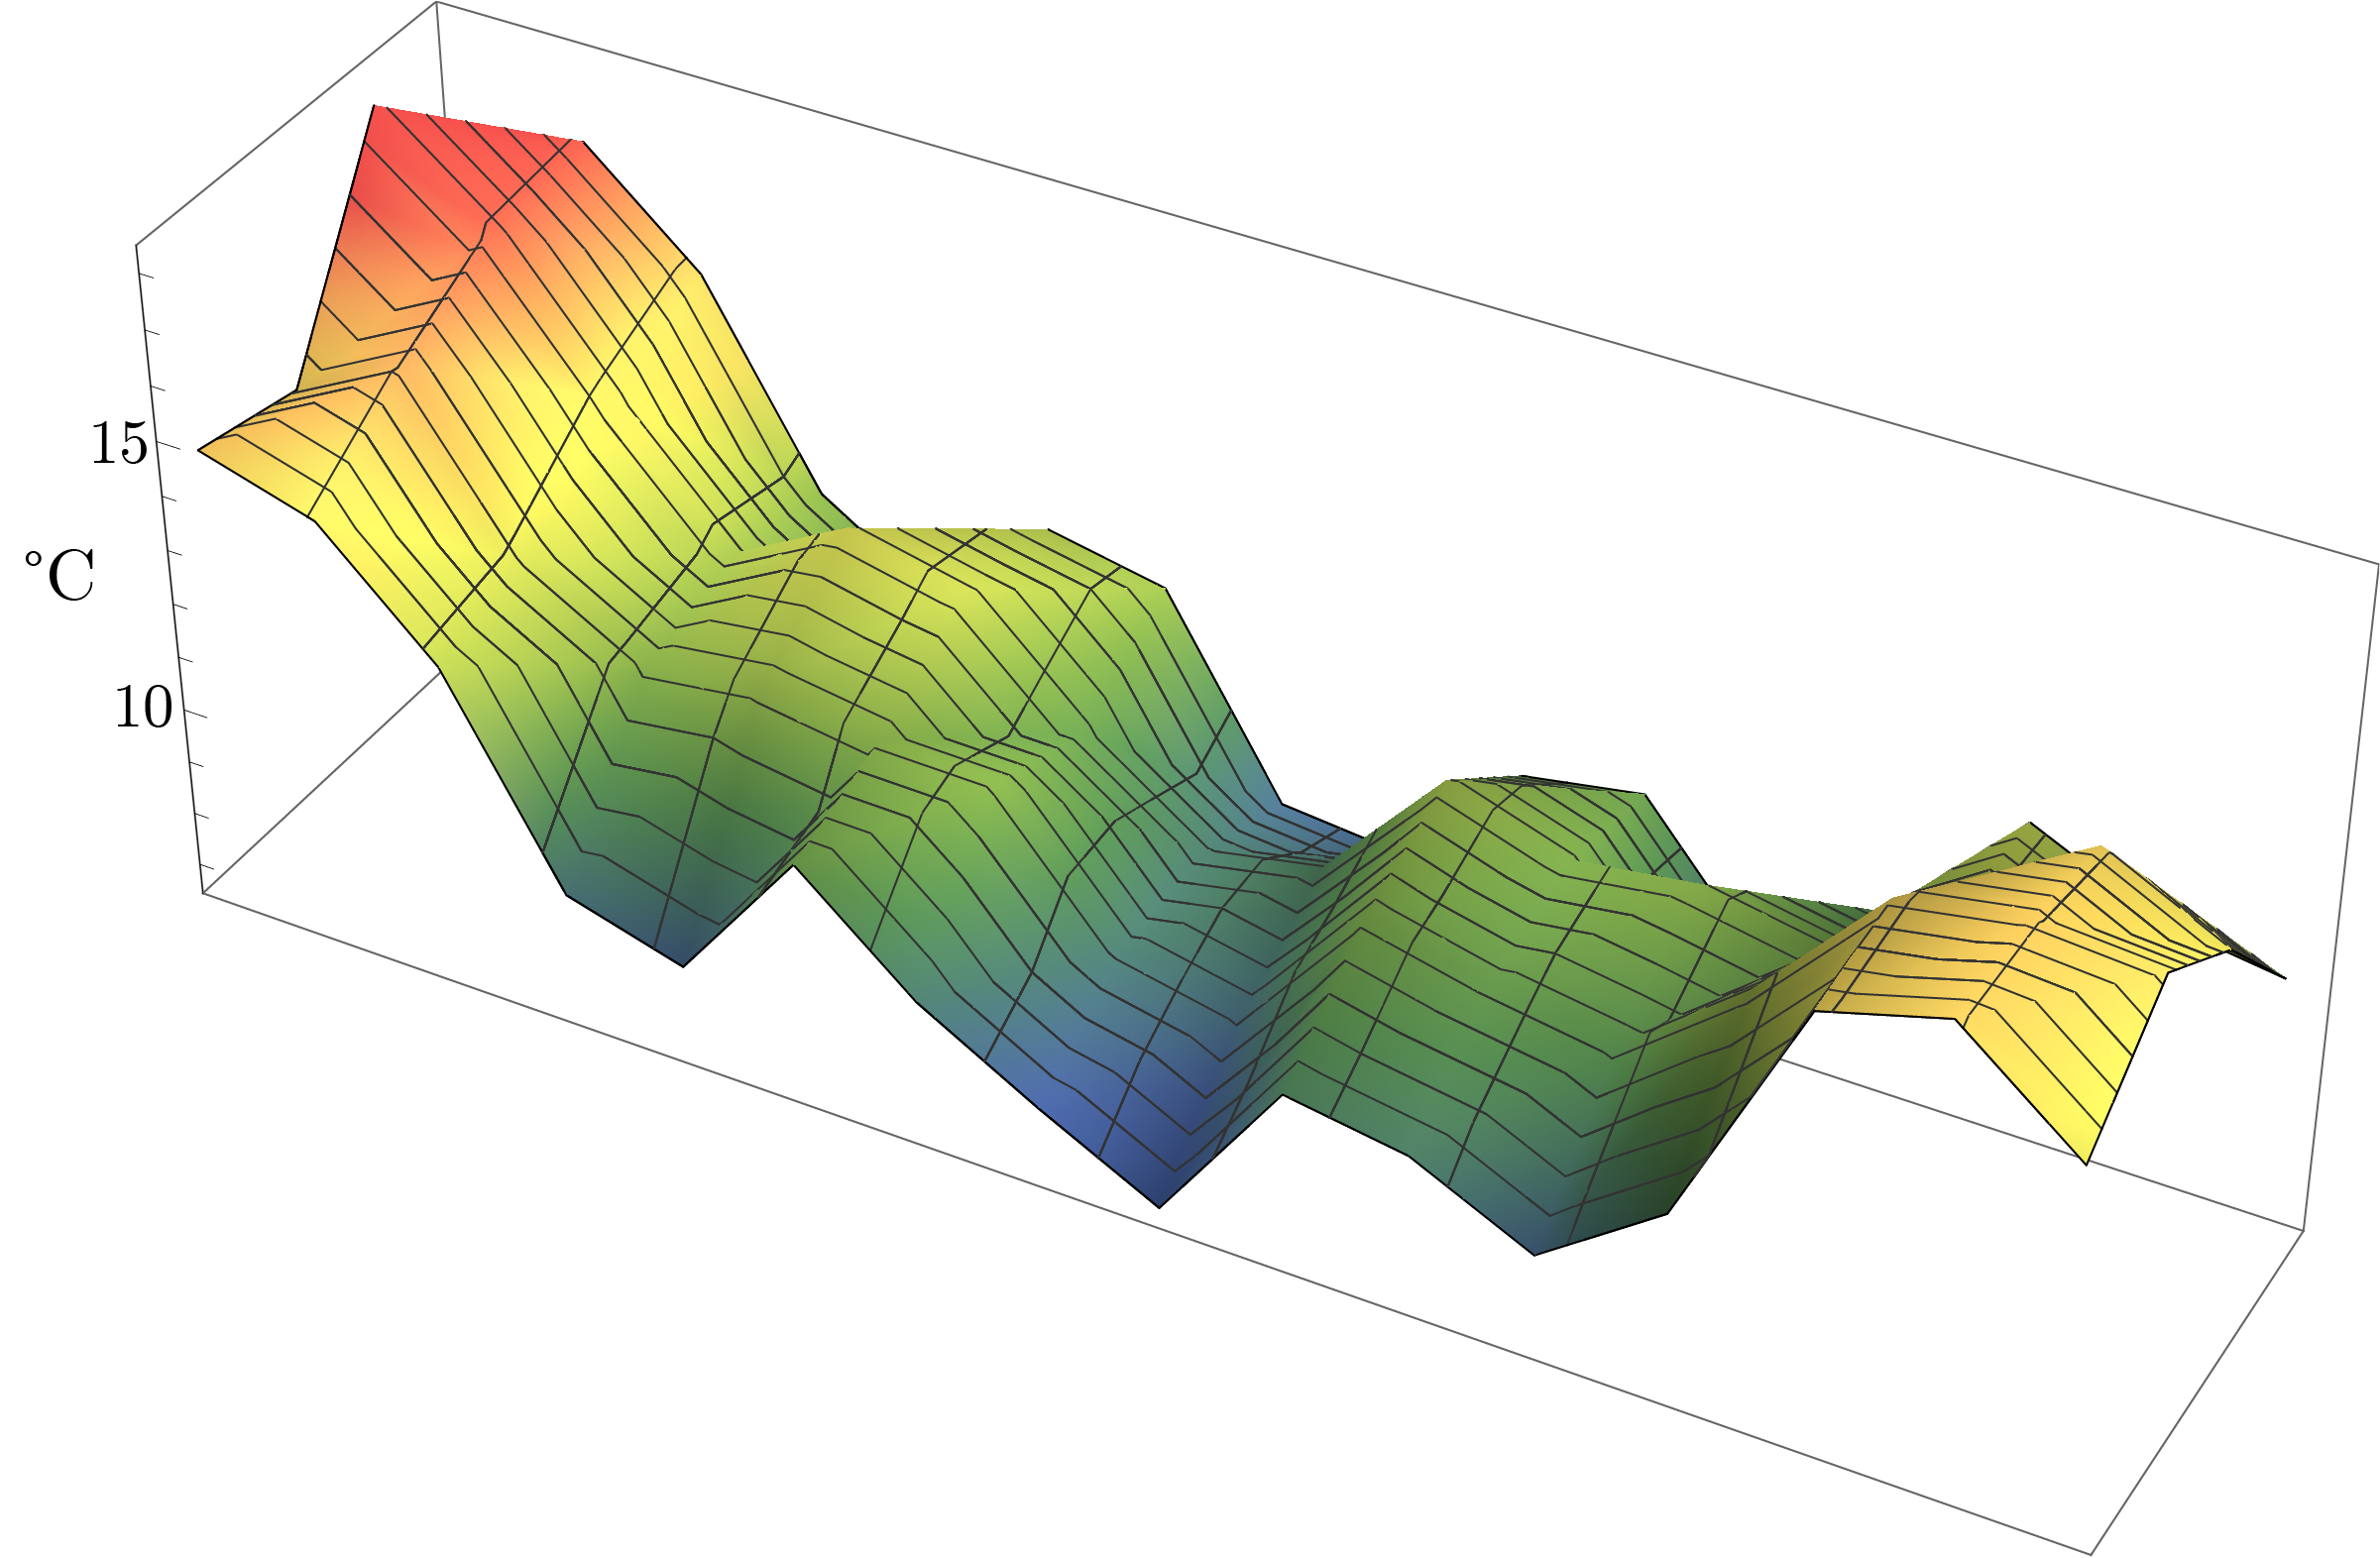
\includegraphics[width=\textwidth]{../diagrams/rest-avg.png}
\caption{Plot of pixel means at rest}
\label{fig:meanplot}
\end{figure}

\begin{figure}
\centering
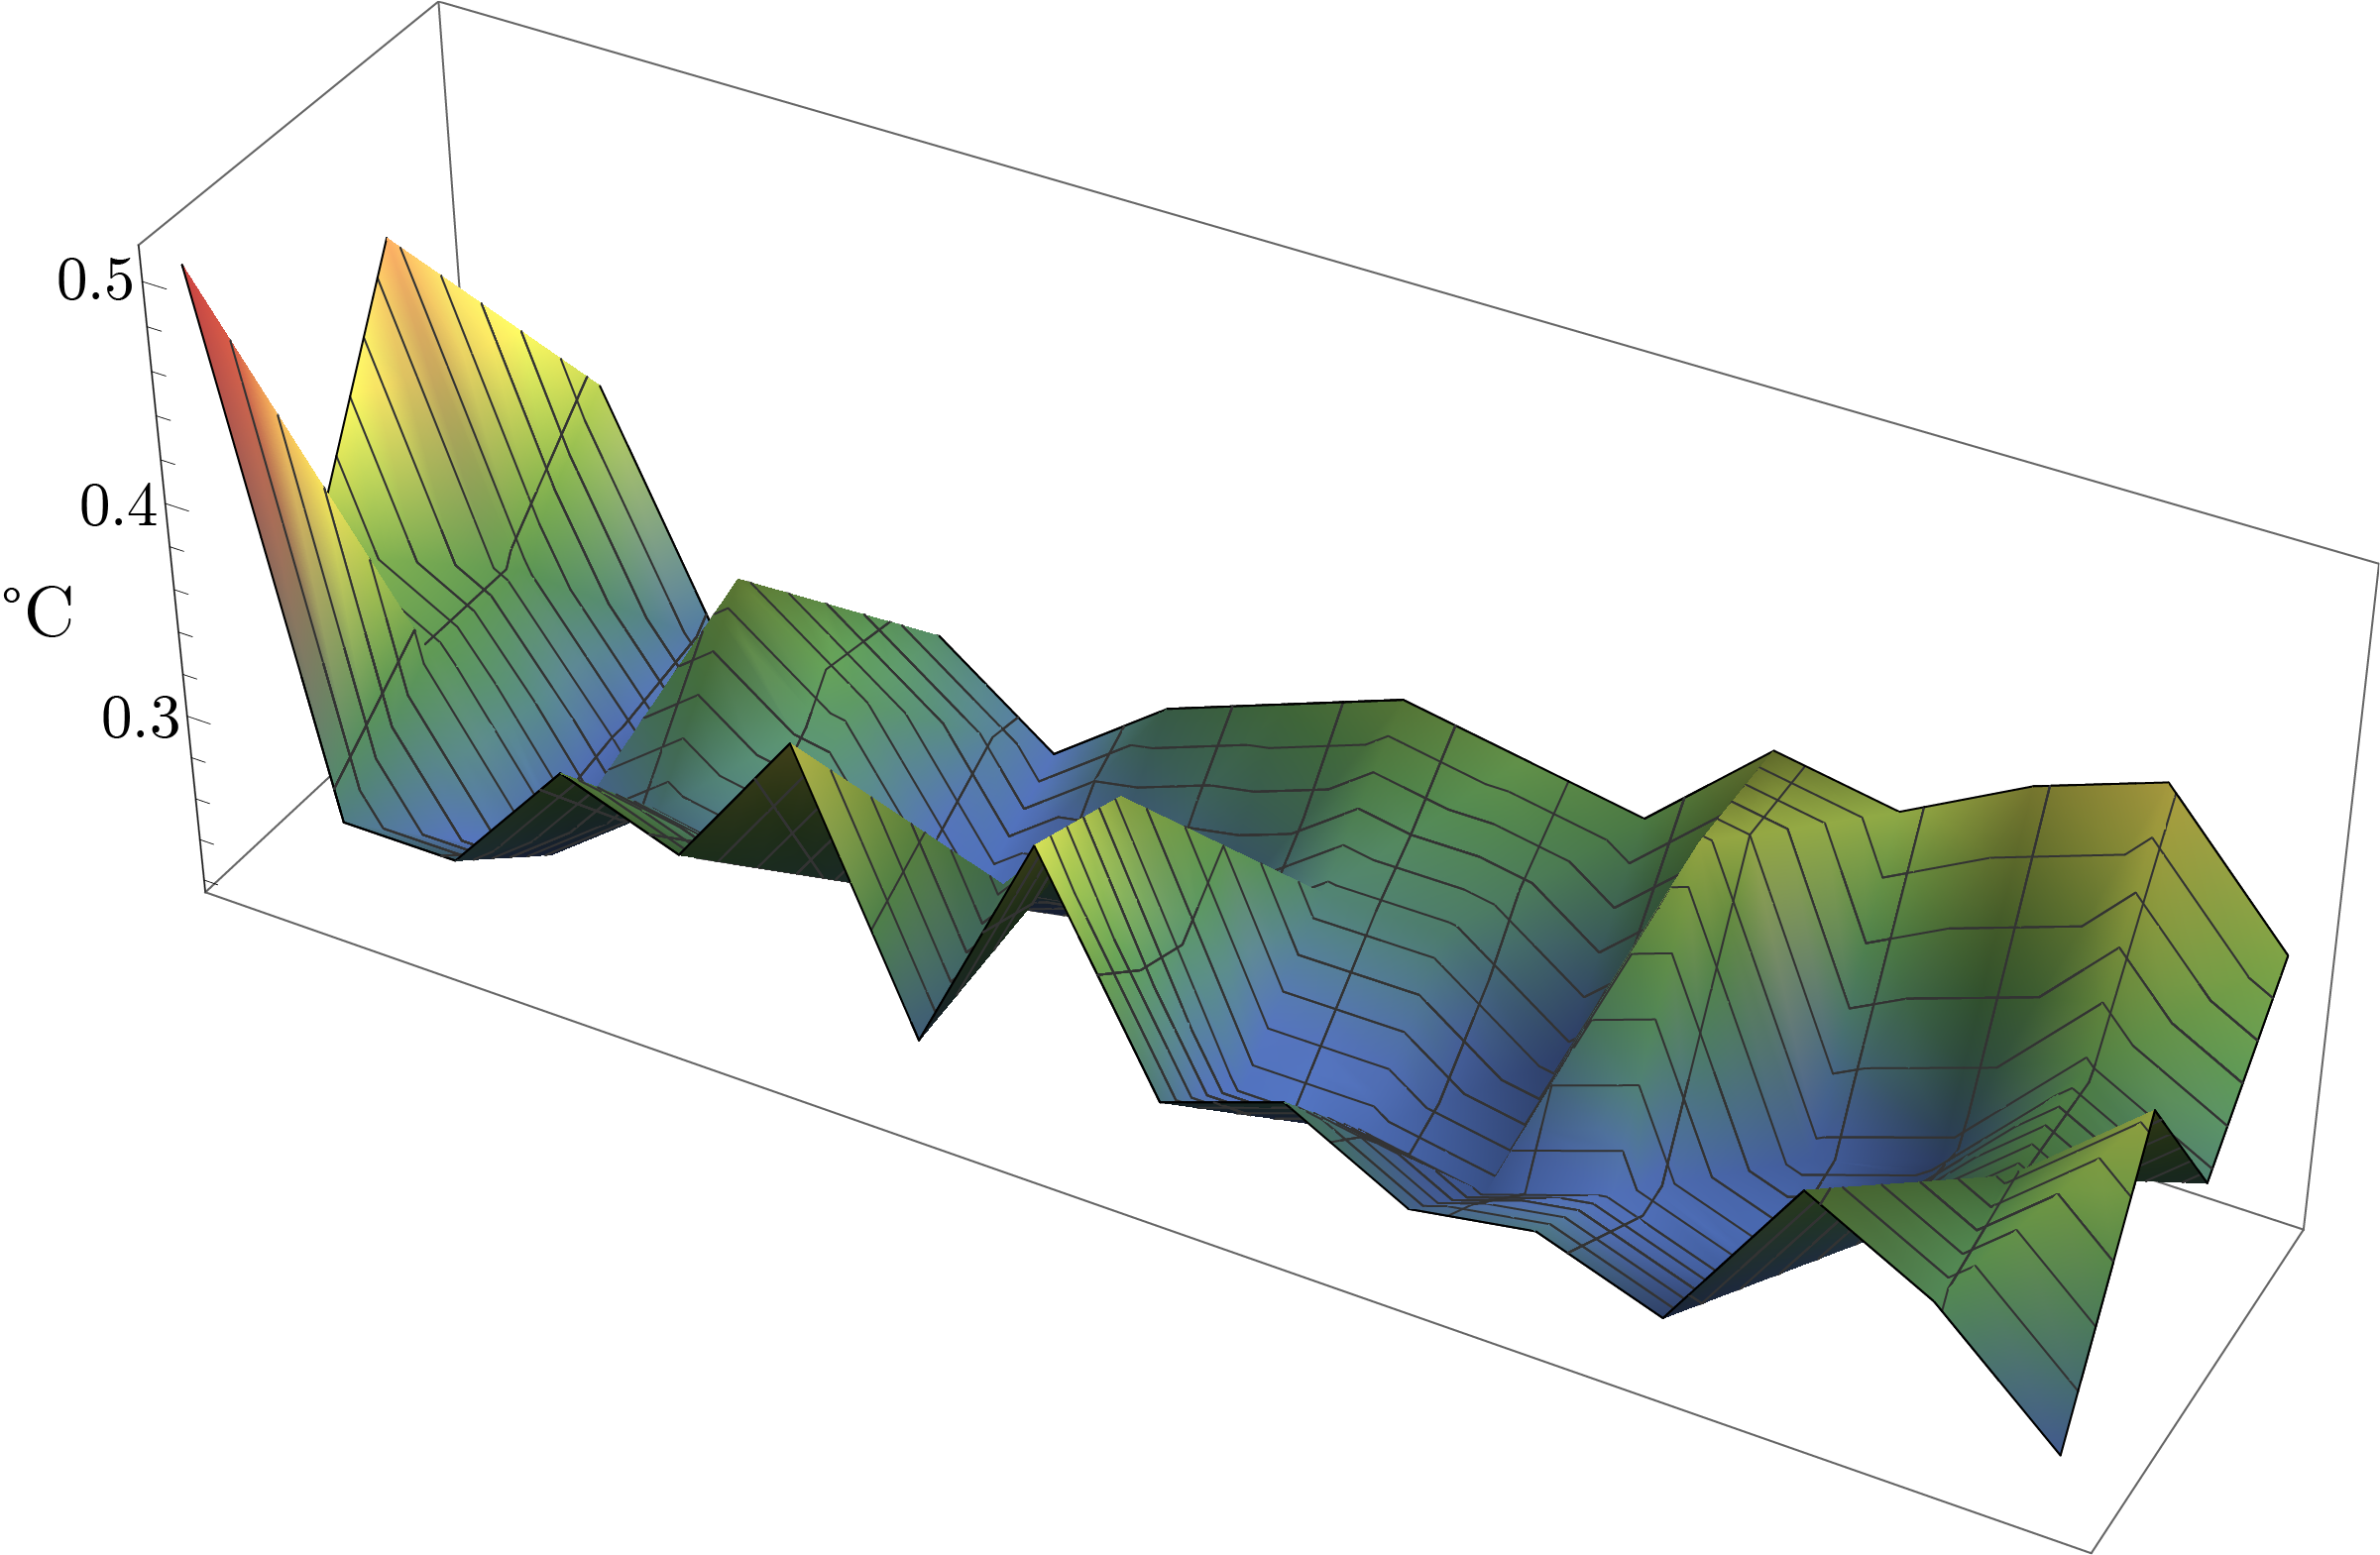
\includegraphics[width=\textwidth]{../diagrams/rest-stddev.png}
\caption{Plot of pixel standard deviations at rest}
\label{fig:stdplot}
\end{figure}


\subsection{Noise}

One of the primary features of the \mlx is the ability to sample the thermal data at a variety of sample rates between 0.5Hz and 512Hz. It was noted in preliminary experimentation that a higher sample rate appeared to result in noisier temperature readings. As our experiments focus on separating objects of interest from a thermal background, it is important to determine if this noise would post an issue for our use case.

\Fref{fig:noise} plots one of the central pixels of the sensor in a scenario where it is detecting a background, and when it is viewing a person, at the five different sample rates achievable with the current hardware configuration. We can see in these plots that the data becomes significantly more noisy as the sample rate increases, and we can also conclude that the sensor uses a form of data smoothing at lower sample rates, as the variance in data increases with sample rate. If the sample rate were to increase beyond a certain threshold, it is likely that the ability for the sensing system to disambiguate between objects of interest and the background would diminish.

\begin{figure}
  \centering
  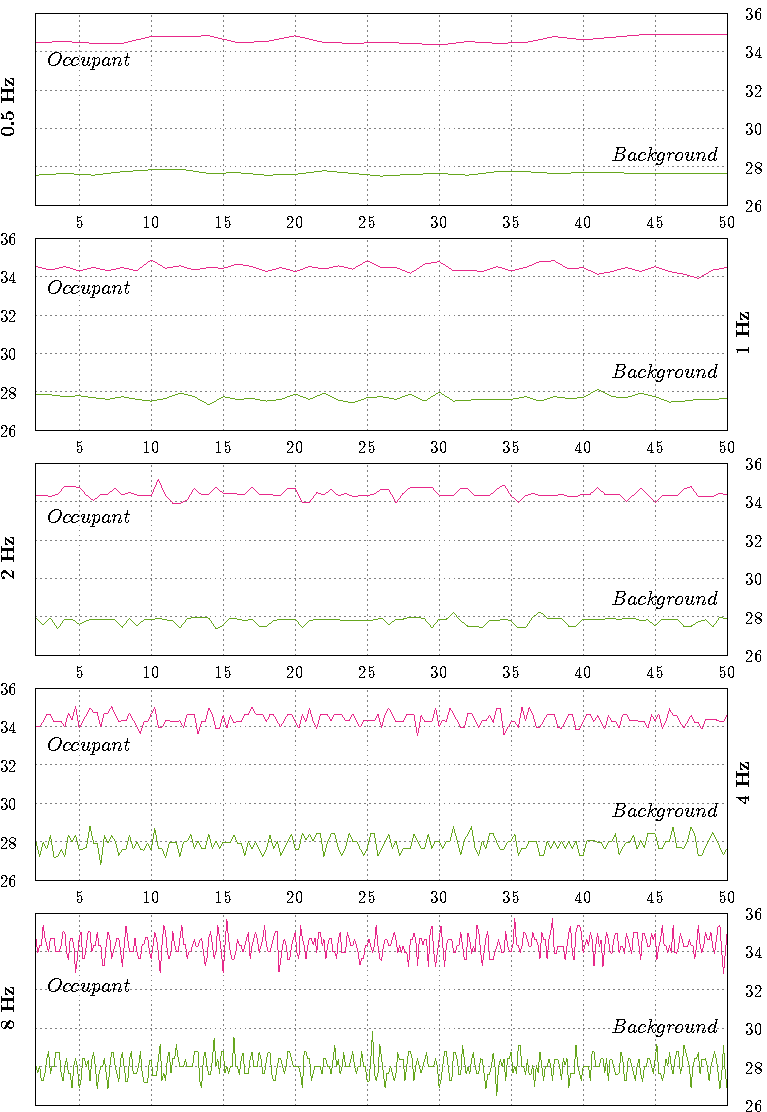
\includegraphics[width=0.95\textwidth]{../diagrams/noise-graph.pdf}
  \caption{Noise levels of occupants and background at various sampling speeds}
  \label{fig:noise} % TODO: Update graph with newer one with std invo
\end{figure}

In the 0.5Hz case, the third standard deviation above background ($3\sigma_b$) is $6.4\dc$ below the minimum occupant value ($\mathrm{min}(o)$) detected. As the noise increases, this gap slowly decreases, with $5.75\dc$ for 1Hz, $5.53\dc$ for 2Hz, $4.48\dc$ for 4Hz, and finally $3.15\dc$ for 8Hz. In none of these cases is $3\sigma_b \ge \mathrm{min}(o)$, which would completely rule that sample rate out.

Based on the data, noise will not pose any issue as the slowest sampling rate of 0.5Hz is sufficient for the system's needs, and shows a sufficiently large gap between occupant and background temperatures. Higher sample rates are unnecessary as occupancy estimations at a sub-second level present little additional value.

% TODO: Signal to noise ratio calculations

\subsection{Sensitivity}
\label{subsec:sensitivity}

The \mlx is a sensor composed of 64 independent non-contact digital thermopiles, which measure infrared radiation to determine the temperature of objects. While they are bundled in one package, the sensor's block diagram discussed previously (\Fref{fig:exps:blockdia}) shows that they are in fact wholly independent sensors placed in a grid structure. This has important effects on the properties of the data that the \mlx produces. 

\Fref{fig:hotmotion} shows a smoothed temperatures graph of six of the sensor's central pixels as a hot object is moved from left to right at an approximately constant speed. One of the most interesting phenomena in this graph is the variability of the object's detected temperature as it moves ``between'' two different pixels; there is a noticeable drop in the objects detected temperature. Each pixel appears to exhibit a bell-curve like line, with the detected temperature increasing from the baseline and peaking as the object enters the center of the pixel, and the detected temperature similarly decreasing as the object leaves the center. 

This phenomenon has several possible causes. One likely explanation is that each individual pixel detects objects radiating at larger angles of incidence to be colder than they actually are: As the object enters a pixel's effective field of view, it will radiate into the pixel at an angle that is at the edge of the pixel's ability to sense, with this angle slowing decreasing until the hot object is directly radiating into the pixel's sensor, causing a peak in the temperature reading. As the object leaves the individual element's field of view, the same happens in reverse.

While interesting, this phenomenon has little consequence to the effectiveness of the techniques used, as in experimental conditions the sensor will not be sufficiently distant that humans could be detected as single pixels.

\begin{figure}
\centering
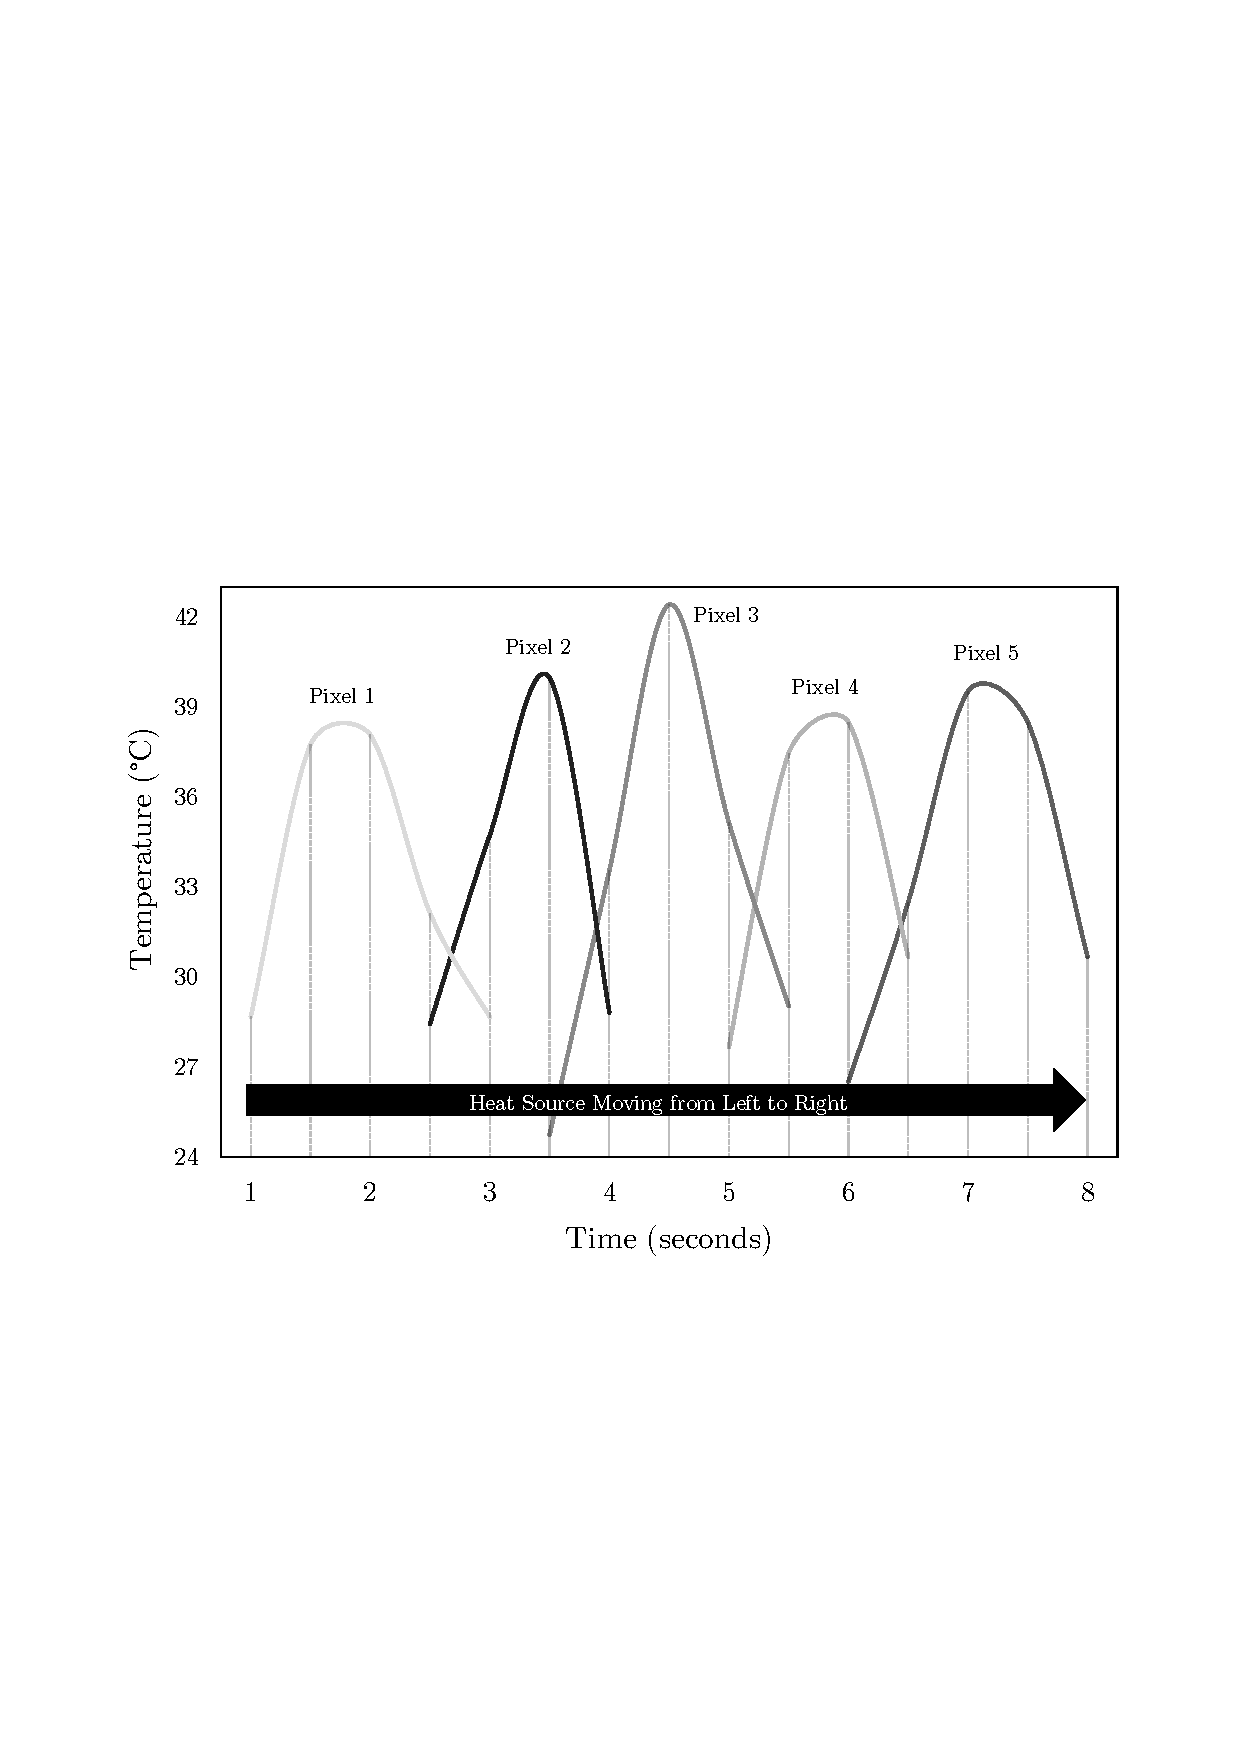
\includegraphics[width=0.9\textwidth]{../diagrams/03_hot_water_top_row_modified.pdf}
\caption{Measure of top-centre 6 \mlx pixels as hot object moves across (smoothed)}
\label{fig:hotmotion}
\end{figure}

% ASK: Smoothed lines ok?

\section{Classification Accuracy}

With a greater understanding of the prototype's caveats, it is now possible to gather both thermal and visual data in a synchronized format. This data can be collected and used to determine the effectiveness of the occupant counting algorithms used. Due to the prototype's technical similarly to Thermosense \cite{beltran2013thermosense}, a similar set of experimental conditions will be used, with a comparison against Thermosense being used as a benchmark. To this end, several experiments were devised, each of which had its data gathered and processed in accordance with the same general process, outlined in \Fref{fig:methods:flowchart} and discussed in more detail in this section.

\begin{figure}
\centering
\begin{tikzpicture}[node distance=1.7cm]
\node (raw) [circ] {Raw \linebreak Data};
\node (step1) [box, right=of raw, text width=4cm, minimum width=4cm] {1. Image \linebreak Capture on RPi \linebreak \texttt{cap\_pi\_synced.py}};
\node (frames) [circ, below=of step1] {Captured Images};
\node (step2) [box, right=of frames] {2. Data Labeling \linebreak \texttt{tagging.py}};
\node (truth) [circ, below=of step2] {Per-Frame Truth};
\node (step3) [box, left=of truth] {3. Feature Extraction \linebreak \texttt{weka\_export.py}};
\node (csv) [circ, below=of step3] {CSV File};
\node (step4) [box, below=of csv] {4. Weka Classification \linebreak \texttt{run\_flow.py}};
\node (results) [circ, right=of step4] {Weka Results};

\draw [line,->] (raw) -- (step1);
\draw [line,->] (step1) -- (frames);
\draw [line,->] (frames) -- (step2);
\draw [line,->] (step2) -- (truth);
\draw [line,->] (truth) -- (step3);
\draw [line,->] (step3) -- (csv);
\draw [line,->] (csv) -- (step4);
\draw [line,->] (step4) -- (results);

\draw [line,->] (frames) -- (step3);
\end{tikzpicture}
\caption{Visualization of processing steps}
\label{fig:methods:flowchart}
\end{figure}

\subsection{Data gathering}
As the camera and the Arduino are directly plugged into the Raspberry Pi, all data capture is performed on-board through SSH, with the data being then copied off the Pi for later processing. To perform this capture, the main script used is \texttt{cap\_pi\_synced.py}.

\texttt{cap\_pi\_synced.py} takes two parameters on the command line; the name of the capture output, and the number of seconds to capture. The script initializes the \texttt{picamera} library, then passes a reference to it to the \texttt{capture\_synced} function within the \texttt{Visualizer} class. The class will then handle sending commands to the Arduino to capture data in concert with taking still frames with the Raspberry Pi's camera.

When the script runs, it creates a folder with the name specified, storing both the thermal capture inside a file named \texttt{output\_thermal.hcap}, and a sequence of files with the format \texttt{video-\%09d.jpg} corresponding to each visual capture frame.

\subsection{Data labeling}
\label{subsec:datalabelling}
Once this data capture is complete, the data is copied to a computer with GUI support for labeling. The utility \texttt{tagging.py} is used for this stage. This script is passed the path to the capture directory, and the number of frames at the beginning of the capture that are guaranteed to contain no motion. This utility will display frame by frame each visual and thermal capture together, as well as the computed feature vectors (based on a background map created from the first $n$ frames without motion).

The user is then required to press one of the number keys on their keyboard to indicate the number of people present in this frame. This number will be recorded in a file called \texttt{truth} in the capture's directory. The next frame will then be displayed, and the process continues. This utility enables the quick input of the ground truth of each capture, which is necessary for the classification stage.

\subsection{Feature extraction and data conversion}
% TODO: Explain classification

Once the ground truth data is available, it is now possible to utilize the data to perform various classification tests. For this, we use version 3.7.12 of the open-source Weka toolkit \cite{Weka}, which provides easy access to a variety of machine learning algorithms and the tools necessary to analyze their effectiveness.

We collate and export the ground truth and extracted features from multiple captures to a Comma Seperated Value (CSV) file for processing with Weka. \texttt{weka\_export.py} takes two parameters, a comma-separated list of different experiment directories to pull ground truth and feature data from, and the number of frames at the beginning of each capture that can be considered as ``motionless.'' With this information, a CSV-file file is generated.

\subsection{Running Weka Tests}
Once the CSV file is generated, it is then possible process this file through Weka. Weka provides a variety of algorithms. We choose algorithms based on those present in the Thermosense paper \cite{beltran2013thermosense}, as well others that provide a broad spread of classification techniques. These algorithms are discussed in detail in \Fref{sec:classification}. The Weka parameters used for each of these algorithms can be seen in \Fref{tab:methods:params}.

\begin{table}[h]
\centering
\begin{tabular}{|p{40mm}|p{20mm}|p{70mm}|}
\hline
\textbf{Type} & \textbf{Attribute} & \textbf{Weka Class} \& \textbf{Parameters} \\ \hline

{Neural Network \newline (ANN)} & {Nominal, \newline Numeric} & \texttt{weka.classifiers.functions\newline.MultilayerPerceptron \newline -L 0.3 -M 0.2 -N 500 -V 15 \newline -S 0 -E 20 -H 5} \\ \hline

{$k$-nearest Neighbors \newline (KNN)} & Nominal, \newline Numeric & \texttt{weka.classifiers.lazy.IBk \newline -K 5 -W 0 -F \newline -A "weka.core.neighboursearch\newline.LinearNNSearch -A \textbackslash"weka.core\newline.EuclideanDistance \newline -R first-last\textbackslash""} \\ \hline

Naive Bayes & Nominal & \texttt{weka.classifiers.bayes.NaiveBayes} \\ \hline

{Support Vector \newline Machine (SVM)} & Nominal & \texttt{weka.classifiers.functions.SMO \newline -C 1.0 -L 0.001 -P 1.0E-12 \newline -N 0 -V -1 -W 1 \newline -K "weka.classifiers.functions\newline.supportVector.PolyKernel \newline-C 250007 -E 1.0"} \\ \hline

Decision Tree & Nominal & \texttt{weka.classifiers.trees.J48 \newline -C 0.25 -M 2} \\ \hline

Entropy Distance & Nominal, \newline Numeric & \texttt{weka.classifiers.lazy.KStar \newline -B 20 -M a} \\ \hline % TODO: Check that entropy distance

Linear Regression & Numeric & \texttt{weka.classifiers.functions\newline.LinearRegression \newline -S 0 -R 1.0E-8} \\ \hline

0-R & Nominal, \newline Numeric & \texttt{weka.classifiers.rules.ZeroR} \\ \hline
\end{tabular}
\caption{Weka parameters used for classifications}
\label{tab:methods:params}
\end{table}

To help maximize the efficiency of the classification tasks, we use the Weka's Knowledge Flow interface, which provides a drag-and-drop method of creating complex input and output schemes involving multiple different classification algorithms. We generate an encompassing flow that accepts an input CSV file of the raw data, and performs all numeric and nominal classification at once, returning a text file with the results of each of the different classification techniques run. The Knowledge Flow's structure can be seen in \Fref{chap:knowledgeflows}. To further automate this, a Jython script, \texttt{run\_flow.py} is used to call the flow through Weka's Java API. After this is complete, the script then runs a series of regular expressions on the output text data to generate a summary CSV file with the relevant statistical values.

For those tests that are ``nominal,'' the \texttt{npeople} attribute was interpreted as nominal using the ``NumericToNominal'' filter, which creates a class for each value detected in \texttt{npeople}'s columns. For those tests that are ``numeric,'' \texttt{npeople} is left unchanged, as by default all CSV import attributes are interpreted as numeric. For all tests where not specifically stated otherwise, we use 10-fold cross-validation to validate our results.

As the data we are using is based on real experiments, the number of frames which are classified as each class may be unbalanced, which could in turn cause a bias in the classification results. We found that in most cases, the data that most unbalanced the set was that of the zero case, as it was the case most present in the data. As Thermosense previously demonstrated, the use of the \pir alone allows for determining the zero/not-zero case effectively without classification algorithms. Due to this, we attempt to rebalance our dataset by excluding all zero cases from the data Weka receives.

\subsection{Classifier Experiment Set}
% TODO: Justify why pointing down
In our first set of experiments, a scene was devised in accordance with \Fref{fig:exps:3setup} that attempted to sense people from above, as did Thermosense. The prototype was set up on the ceiling, pointing down at a slight angle. For ease of use, the prototype was powered by mains power, and was networked with a laptop for command input and data collection via Ethernet. This set of experiments involved between one and three people being present in the scene, moving in and out in various ways in accordance with the following scripts.

The first four sub-experiments involved people standing;
% ASK: Adequate description
\begin{itemize}
\item Sub-exp 1: One person walks in, stands in center, walks out of frame.
\item Sub-exp 2: One person walks in, joined by another person, both stand there, one leaves, then another leaves.
\item Sub-exp 3: One person walks in, joined by one, joined by another, all three stand there, one leaves, then another, then another.
\item Sub-exp 4: Two people walk in simultaneously, both stand there, both leave simultaneously.
\end{itemize}

The latter five sub-experiments involved people sitting;
\begin{itemize}
\item Sub-exp 5: One person walks in, sits in center, moves to right, walks out of frame.
\item Sub-exp 6: One person walks in, joined by another person, both sit there, they stand and switch chairs, one leaves, then another leaves.
\item Sub-exp 7, 8: One person walks in, joined by one, joined by another, they all sit there, one leaves, one shuffles position, then another leaves, then another. (x2)
\item Sub-exp 9: Two people walk in, both sit there simultaneously, both leave simultaneously.
\end{itemize}

In these experiments people moved slowly and deliberately, making sure there were large pauses between changes of action. The people involved were of average height, wearing various clothing. The room was cooled to 18 degrees for these experiments.

Each experiment was recorded with a thermal-visual synchronization at 1Hz over approximately 60-120 second intervals. Each experiment had 10-15 frames at the beginning where nothing was within the view of the sensor to allow the thermal background to be calculated. Each frame generated from these experiments was manually tagged with the ground truth value of its number of occupants using the tagging script discussed in \Fref{subsec:datalabelling}.

The resulting features and ground truth were combined and exported to CSV allowing Weka to analyze them. This data was analyzed with the feature vectors always being considered numeric data and with the ground truth considered both numeric and nominal. We evaluate the dataset against a set of classification algorithms introduced in \Fref{sec:classification} of our Literature Review.

\begin{landscape}
 \begin{figure}
 \centering
 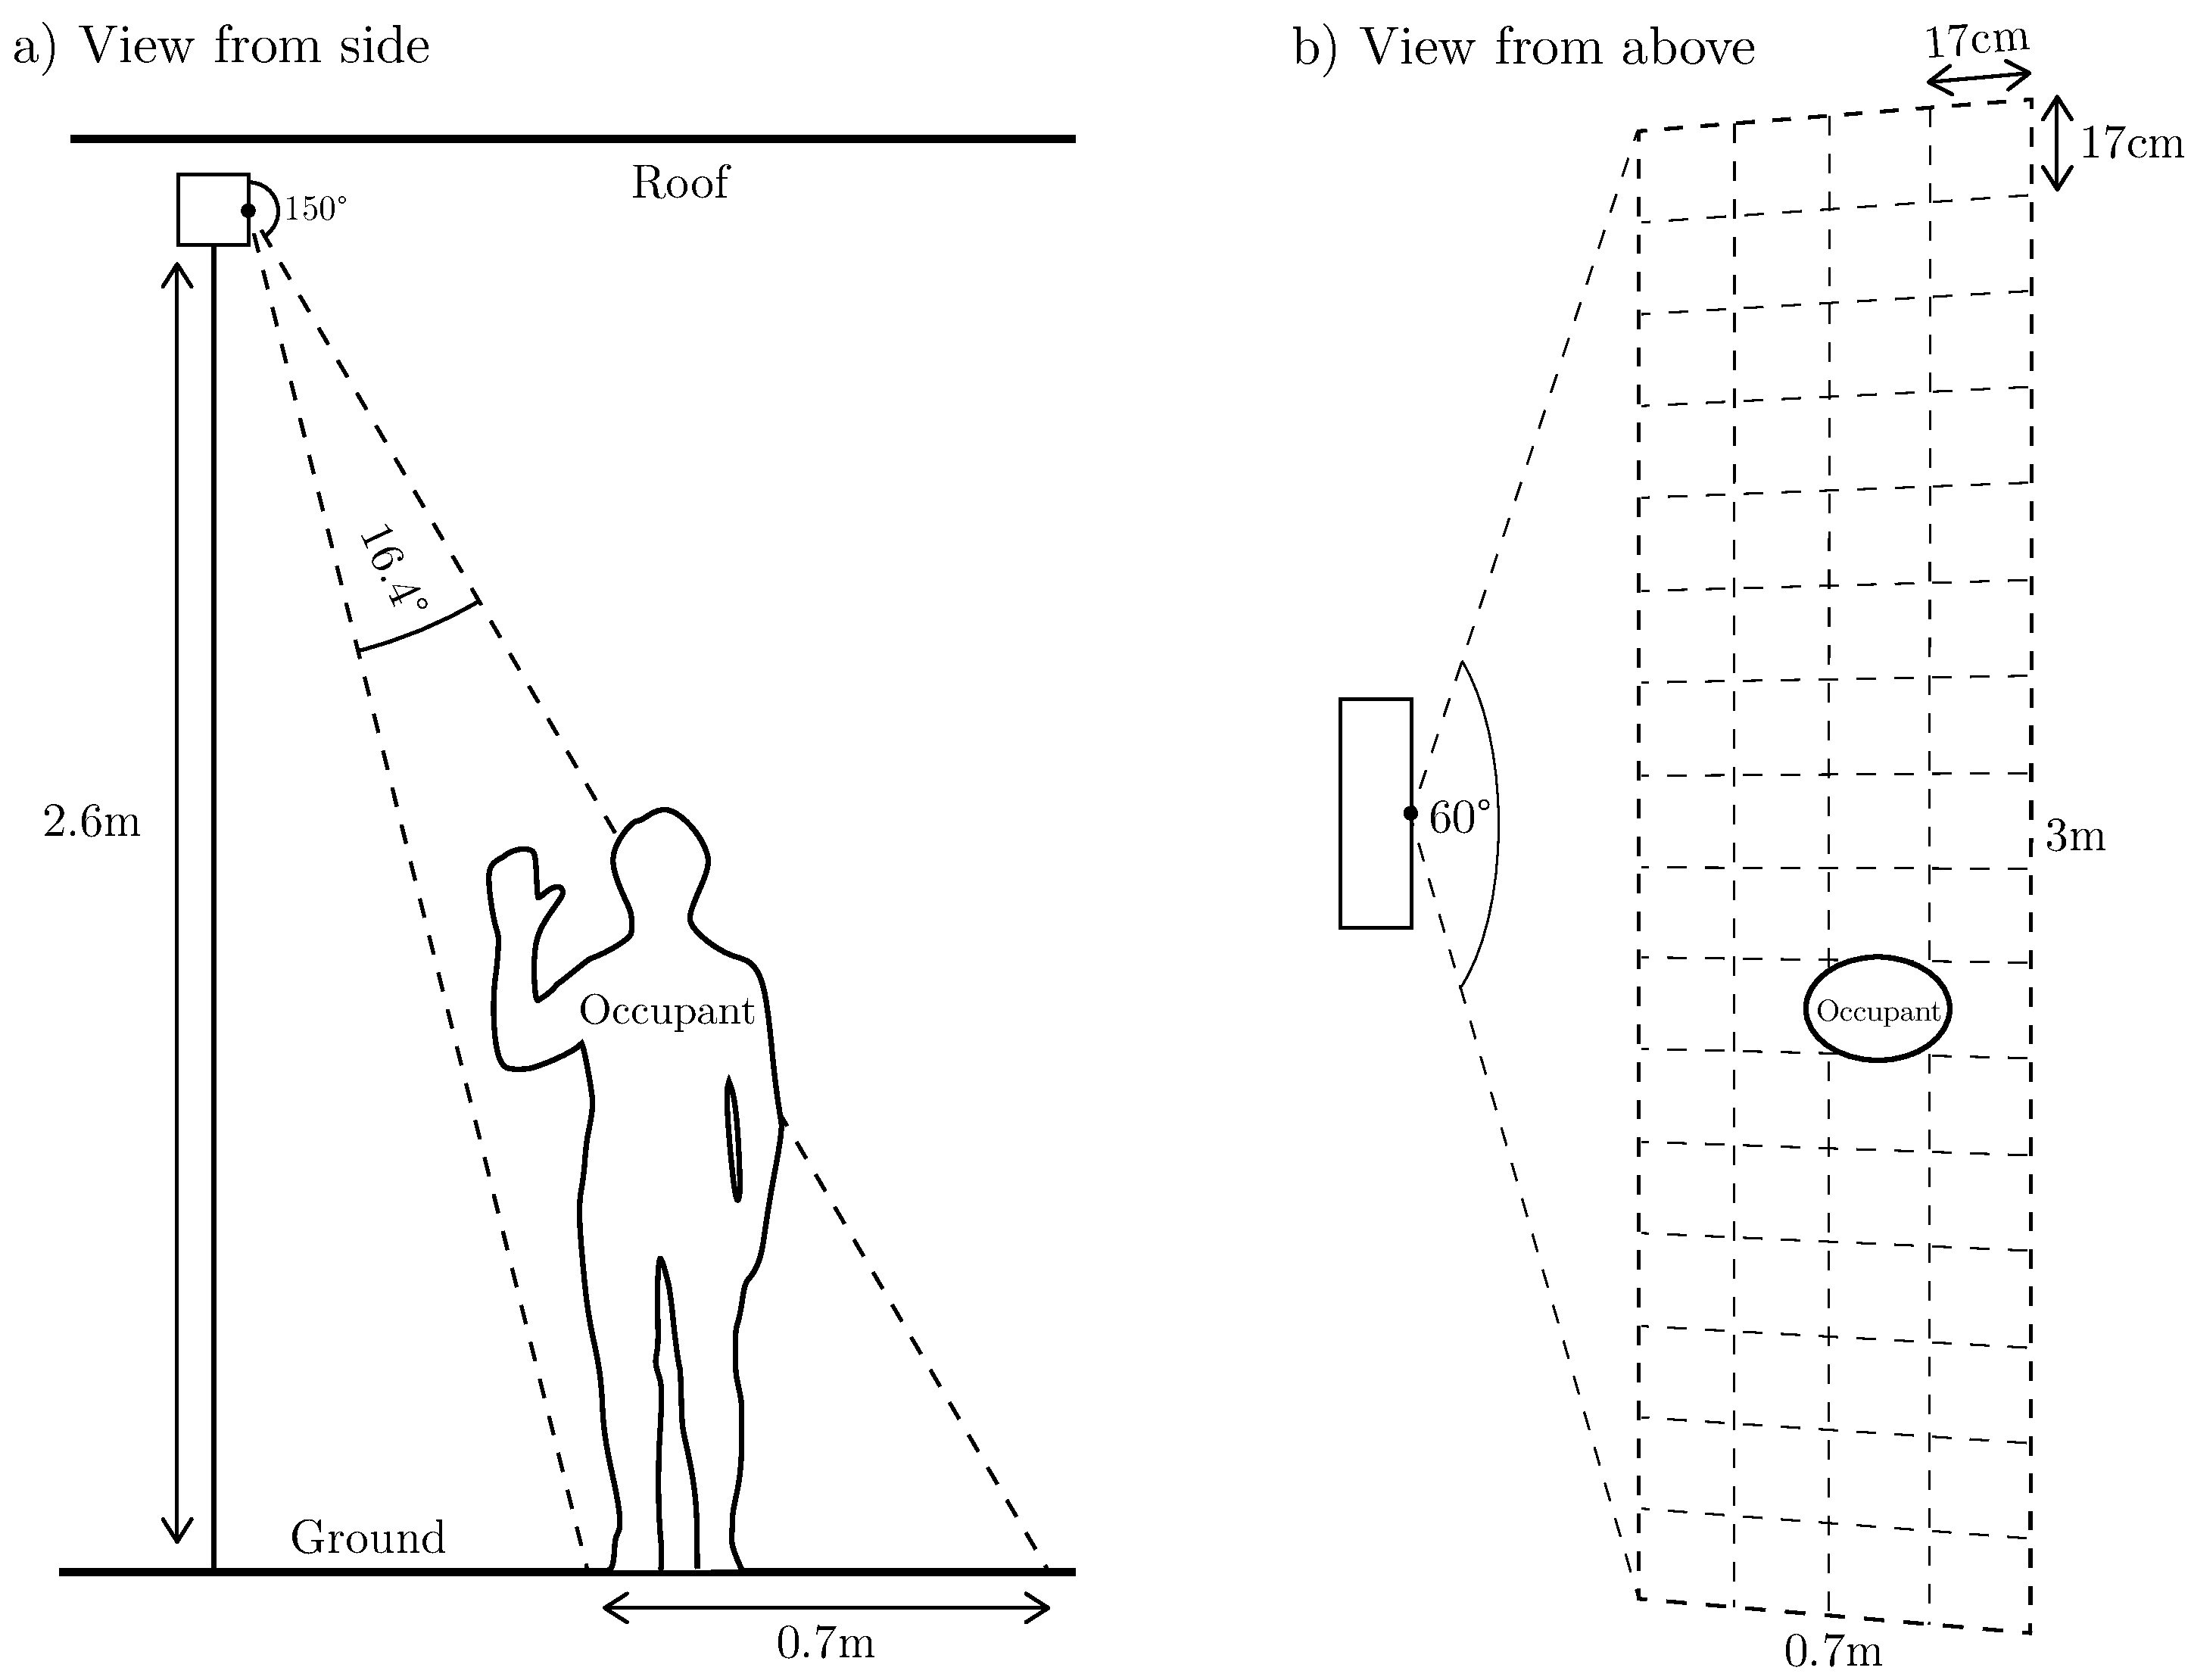
\includegraphics[height=\textheight]{../diagrams/third-exp-setup2.pdf}
 \caption{Classifier Experiment Set Setup (measurements approximate)}
 \label{fig:exps:3setup}
 \end{figure}
\end{landscape}

\section{Results}
\label{sec:results}

\subsection{Classification}
\label{subsec:classification}

Our results (\Fref{tab:results:set1}) show an interesting spread of accuracies between the different tests that were tried. We will analyze the data with reference to two broad categories; those tests replicating Thermosense, and those tests we ourselves proposed.

As discussed previously, significant care was taken to ensure that the same classification parameters were used between our experiments and those performed in Thermosense to provide as accurate as possible a comparison between our results. However, there were some ambiguities with the Thermosense results that have made it more difficult to determine which parameters to choose. In particular, with reference to the $k$-Nearest Neighbours tests (KNN), it was ambiguous within the Thermosense paper as to if they had elected to use a nominal classification or a numeric classification for this data.

Because of this, four tests were performed overall to replicate the Thermosense results; KNN tests for both numeric and nominal representations of data, a Multi-Layer Perceptron numeric test (MLP) and a Linear Regression numeric test (Lin Reg). With these tests we found that our prototype performed consistently poorly when compared with Thermosense. Thermosense reported correlation coefficients ($r$) of around 0.9 for their MLP and Lin Reg tests, however we could not replicate these results, with our best being 0.69 and 0.59 respectively. We were also unable to achieve the low Root Mean Squared Errors (RMSEs) reported by Thermosense, with their RMSEs for KNN, MLP and Lin Reg being 0.346, 0.385 and 0.409 respectively, while ours were 0.364 (KNN Nominal Case), 1.123 (KNN Numeric Case), 0.592 (MLP) and 0.525 (Lin Reg). Our numeric KNN test performed worse than the 0-R benchmark for numeric tests, indicating a very poor result, with it achieving an RMSE of 1.123 vs. the 0-R's 0.651.

For our own proposed nominal classification algorithms, our accuracies were significantly better, and in some cases exceeded the RMSEs reported by Thermosense. Within our dataset, the K* and C4.5 algorithms were most accurate, with accuracies of 82.56\% and 82.39\% respectively. They both achieved RMSEs lower than the best achieved by Thermosense, with their 0.304 and 0.314 a significant improvement on Thermosense's KNN RMSE of 0.346.

Following down the ranking, our nominal MLP performed next best, with an accuracy of 77.14\%, and an RMSE of 0.362, which is slightly higher than Thermosense's best result. Following, the Support Vector Machine (SVM) implementation achieved a relatively poor accuracy of 67.18\% with an RMSE of 0.398, and finally the Naive Bayes (N. Bayes) approach, achieved the worst accuracy of 63.59\% with an RMSE of 0.405. None of these techniques however achieved an RMSE or accuracy worse than our 0-R benchmark, which achieved an RMSE of 0.442 and an accuracy of 49.74\%.

In our sole numeric choice of K*, we found that it achieved a better correlation than any Thermosense technique, with $r = 0.760$. Additionally, its RMSE of 0.423 was also superior.

\begin{table}
\centering
\begin{tabular}{|l|r|r|r|}
\hline
\textbf{Classifier} & \textbf{RMSE} & \textbf{\%} & \textbf{$r$} \\ \hline
\multicolumn{4}{|c|}{Thermosense Actual}                         \\ \hline
KNN$^1$             & 0.346         &             &              \\ \hline
Lin Reg             & 0.385         &             & 0.926        \\ \hline
MLP                 & 0.409         &             & 0.945        \\ \hline
\multicolumn{4}{|c|}{Thermosense Replication}                    \\ \hline
KNN$^1$             & 0.364         & 65.65       &              \\ \hline
MLP                 & 0.592         &             & 0.687        \\ \hline
Lin Reg             & 0.525         &             & 0.589        \\ \hline
KNN$^1$             & 1.123         &             & 0.377        \\ \hline
\multicolumn{4}{|c|}{Numeric}                                    \\ \hline
K*                  & 0.423         &             & 0.760        \\ \hline
0-R                 & 0.651         &             & -0.118       \\ \hline
\multicolumn{4}{|c|}{Nominal}                                    \\ \hline
K*                  & 0.304         & 82.56       &              \\ \hline
C4.5                & 0.314         & 82.39       &              \\ \hline
MLP                 & 0.362         & 77.14       &              \\ \hline
SVM                 & 0.398         & 67.18       &              \\ \hline
N. Bayes            & 0.405         & 63.59       &              \\ \hline
0-R                 & 0.442         & 49.74       &              \\ \hline
\end{tabular}\\
\parbox{220pt}{
$^1$: Included zero in training data \\
\%: Percentage accuracy, for a nominal test \\
$r$: Correlation coefficient, for a numeric test \\
}
\caption{Classifier Experiment Set Results}
\label{tab:results:set1}
\end{table}

\subsection{Energy Efficiency}
\label{subsec:energy}

% TODO: Energy efficiency table

A YZXStudio USB 3.0 Power Monitor was used to measure power consumed by the Pre-Processing and Sensing tier together while experimenting, as in a more advanced prototype, they would be envisioned to be run on battery power. This was done by connecting the Arduino's USB cable to the Monitor, and the Monitor to a computer. It was calculated that the average power consumption was 51~mA at 4.92~volts with a sample rate of 1Hz, while continuously outputting data. This power consumption did not vary significantly between sample rates, with the consumption increasing $<$ 0.8~mA with the sample rate being set to 8Hz.

To determine the draw from the \pir and \iar, we disconnected all sensors from the Arduino, and ran the power measurement again. The same code was run on the Arduino. This time we received a result of 45~mA for 1Hz, and 46~mA for 8Hz. We can then conclude that the sensors themselves draw around 6~mA of power.


  \ifcsdef{mainfile}{}{\bibliography{../references/primary}}
\end{document}
 